% include the figures path relative to the master file
\graphicspath{ {./content/intro/figures/} }

\section{Introduction}
\label{sec:intro}  % \label{} allows reference to this section


Breast cancer is the second most common cancer (1.4 million cases per year, 10.9\% of  diagnosed cancers) after lung cancer, followed by colorectal, stomach, prostate and liver cancers~\cite{Ferlay2010}.
In terms of mortality, breast cancer is the fifth most common cause of cancer death.
However, it is ranked as the leading cause of cancer death among females in both western countries and economically developing countries~\cite{cancerStatistics2011}.

Medical imaging plays an important role in breast cancer mortality reduction, contributing to its early detection through screening, diagnosis, image-guided biopsy, treatment follow-up and suchlike procedures~\cite{smith2003american}.
Although \ac{dm} remains the reference imaging modality for breast cancer screening, \ac{us} imaging has proven to be a successful adjunct image modality~\cite{smith2003american,berg2004diagnostic}.
The main advantage of \ac{us} imaging, opposed to other image modalities, is its discriminative power for visually differentiate solid lesions as benign and malignant~\cite{Stavros:1995p12392}.
\Ac{us} screening contributes to reduce the amount of unnecessary biopsies~\cite{ciatto1994contribution}, which is estimated to be between $65\sim85\%$ of the prescribed biopsies~\cite{yuan2010multimodality}, in favour of a less traumatic short-term \ac{us} screening follow-up~\cite{gordon1995malignant}.

 For all these reasons, there is a growing interest in the medical community to incorporate \ac{us} screening as part of the standard procedure~\cite{biradsus}, which encourages the development of \ac{cad} systems applied to \ac{bus} images.

\Cref{fig:lesions} offers a compact, brief and visual idea of breast's structure, their render in a 2D \ac{bus} image, and which markers are recommended to study in order to produce a diagnosis~\cite{biradsus}.
All these markers either describe the lesion's delineation, or describe the relation between the lesion and the surrounding tissue, which also requires a delineation of the lesion to differentiate between the two.
\footnote{More details regarding the visual cues used by radiologist would be present in the final manuscript as a building block for feature extraction}


\begin{figure}
    \centering
    \begin{subfigure}[b]{0.28\textwidth}
        \centering
        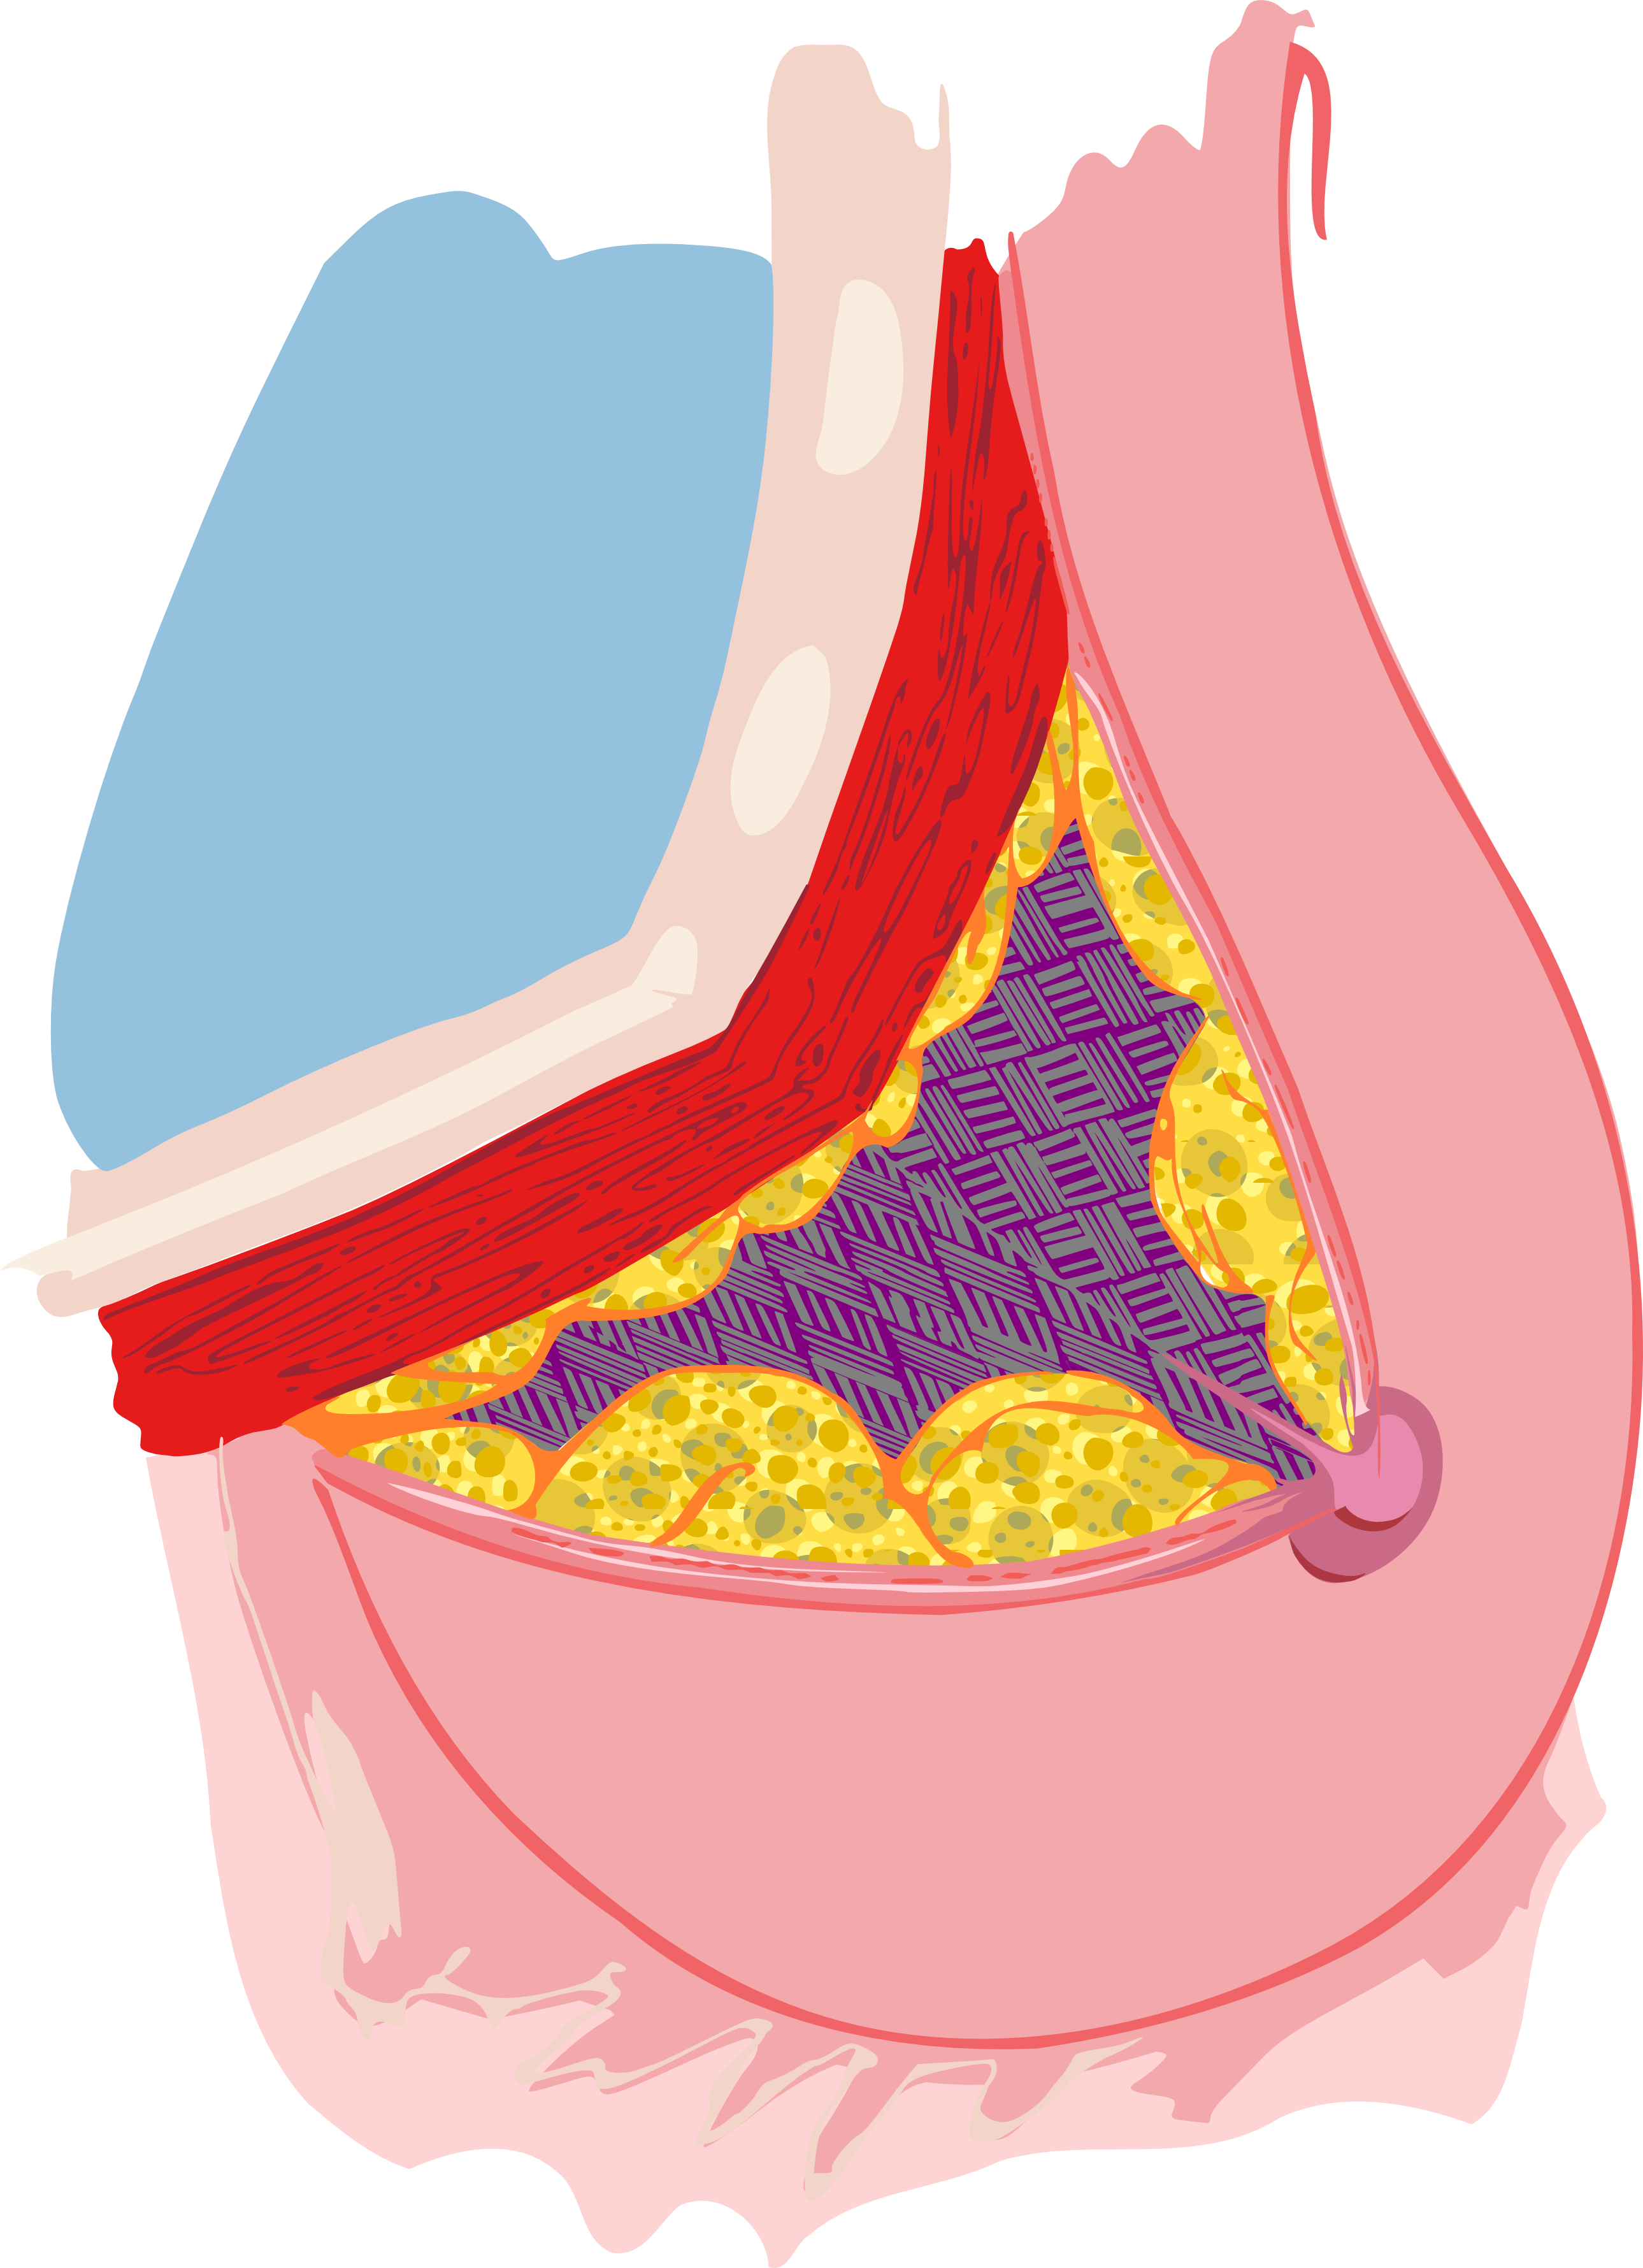
\includegraphics[width=\textwidth]{breast}
        \caption{{\small Breast structure}}
        \label{fig:lesions:breast}
    \end{subfigure}
    \hfill
    \begin{subfigure}[b]{0.25\textwidth}
        \centering
        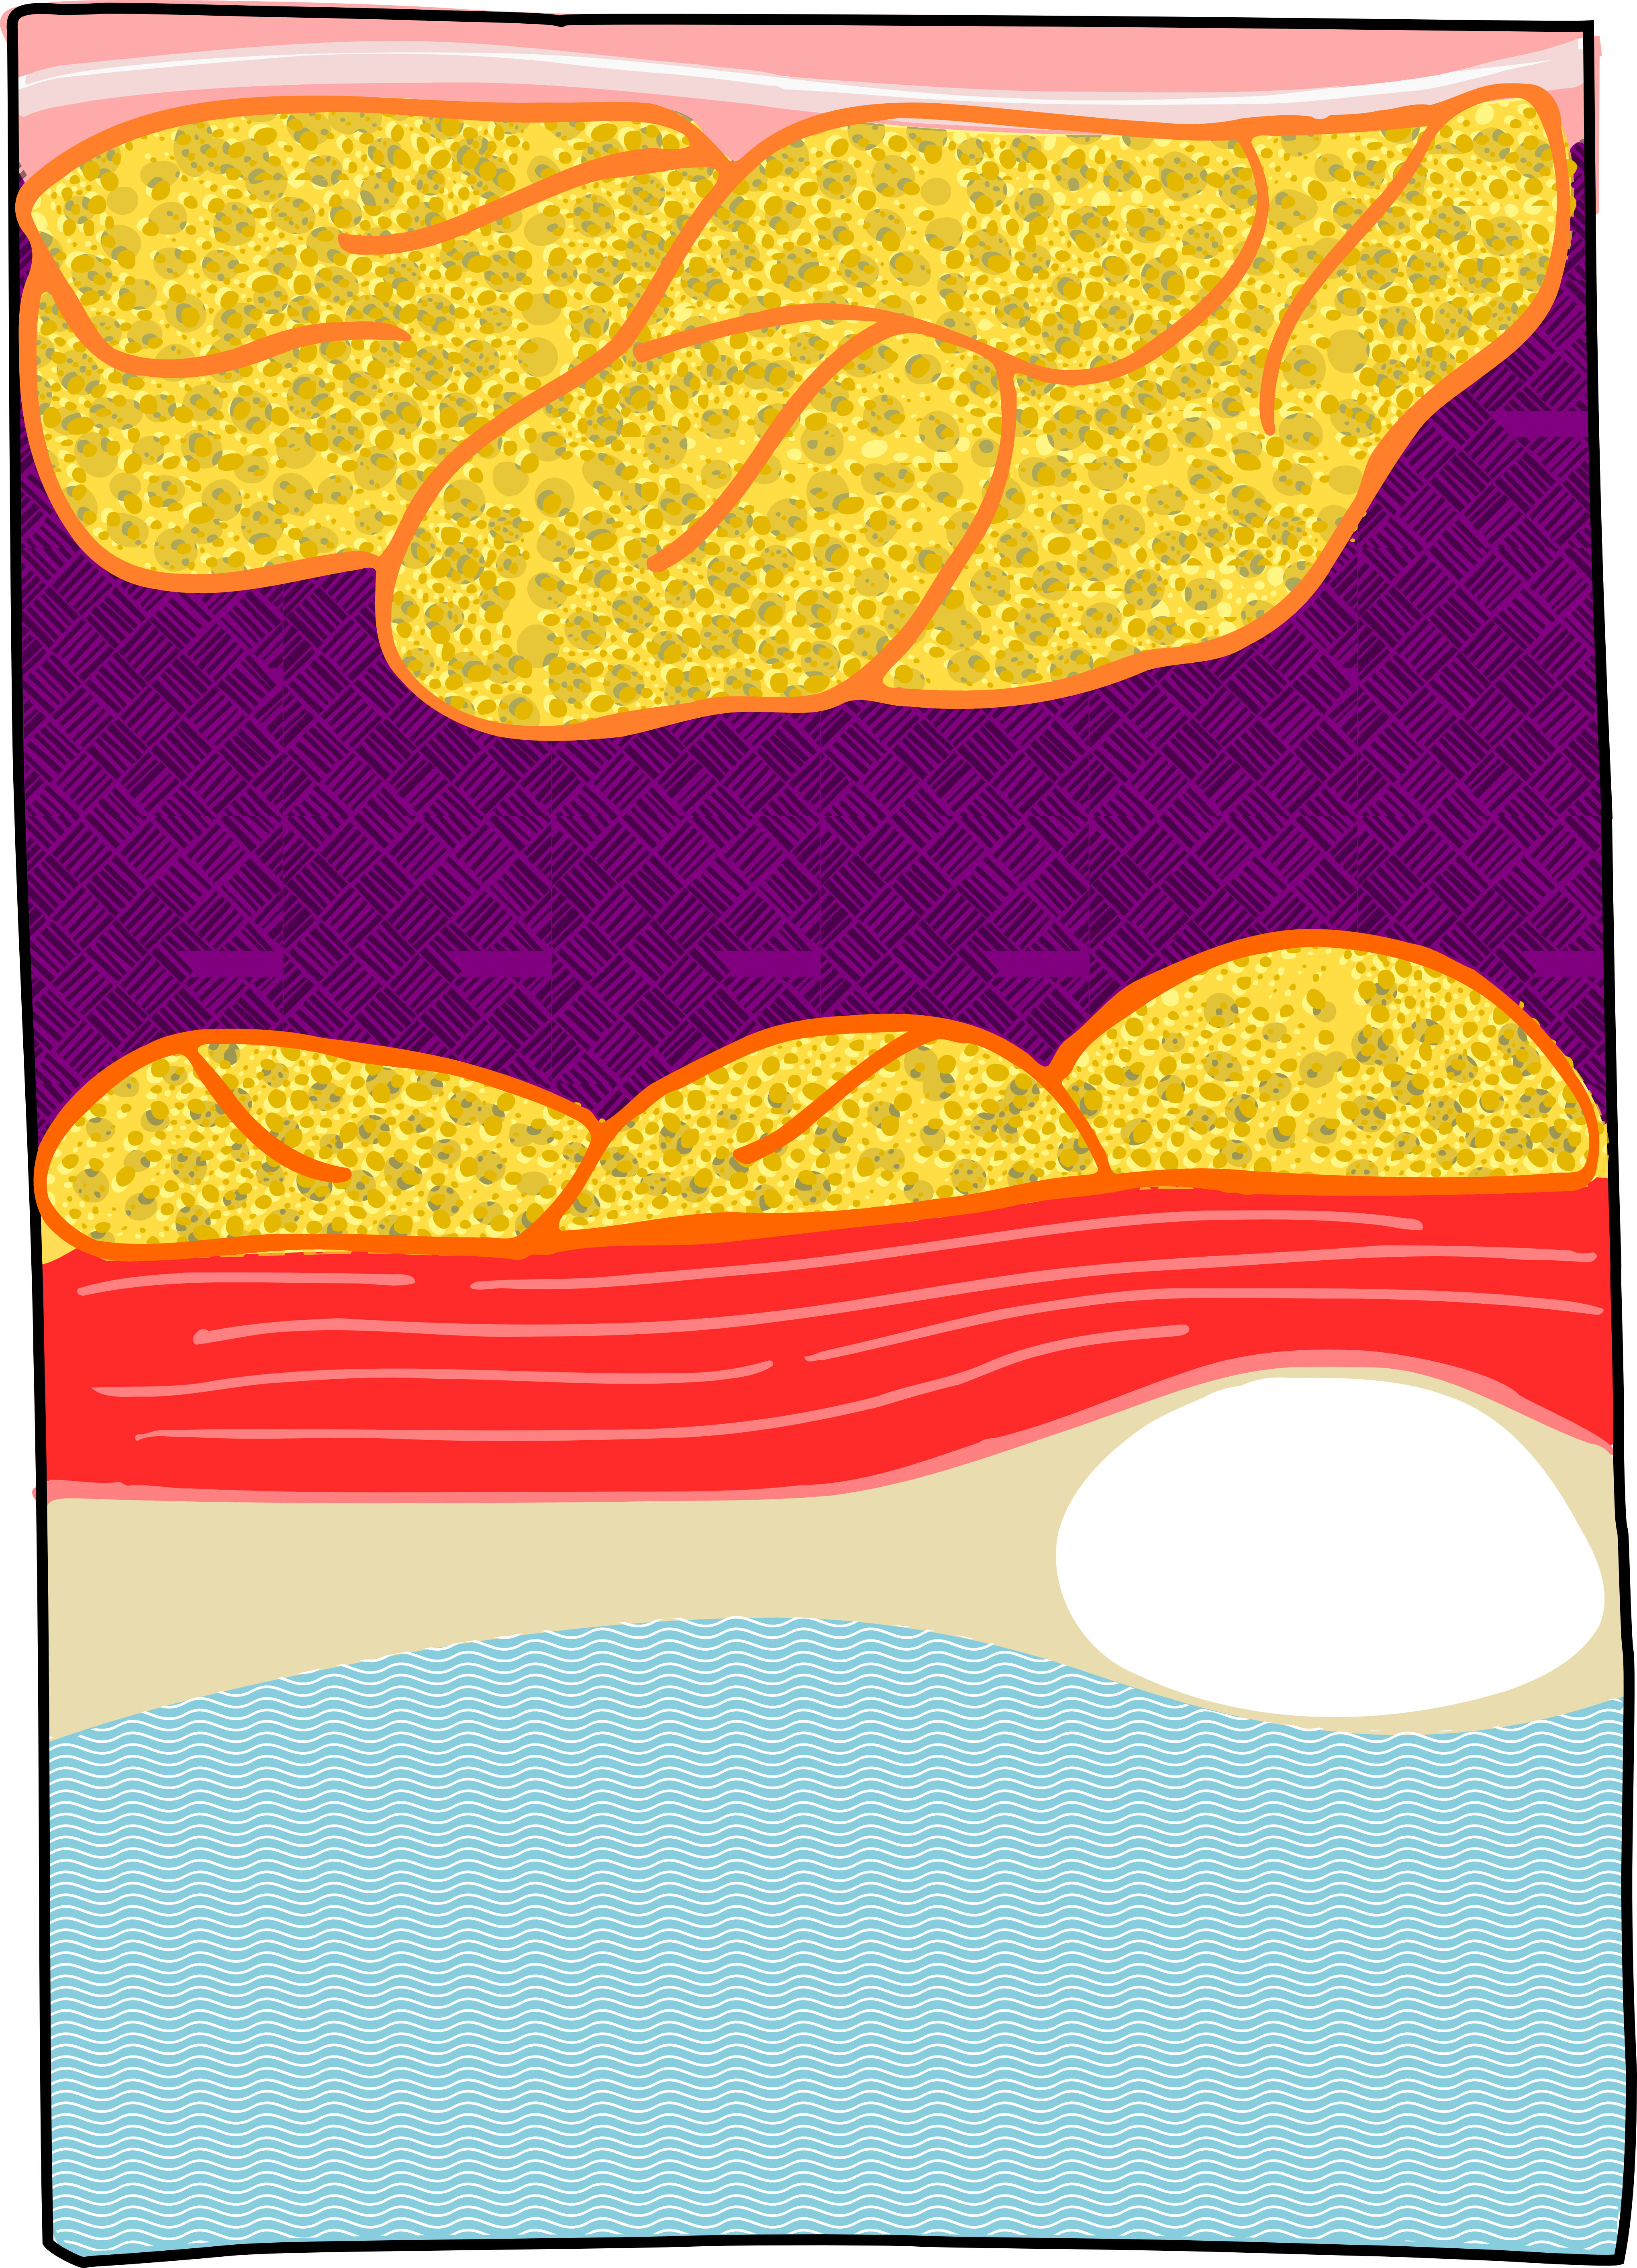
\includegraphics[width=\textwidth]{slice}
        \caption[]%
        {{\small Breast structure location when \ac{us}screening}}
        \label{fig:lesions:slice}
    \end{subfigure}
    \hfill
    \begin{subfigure}[b]{0.4\textwidth}
        \centering
        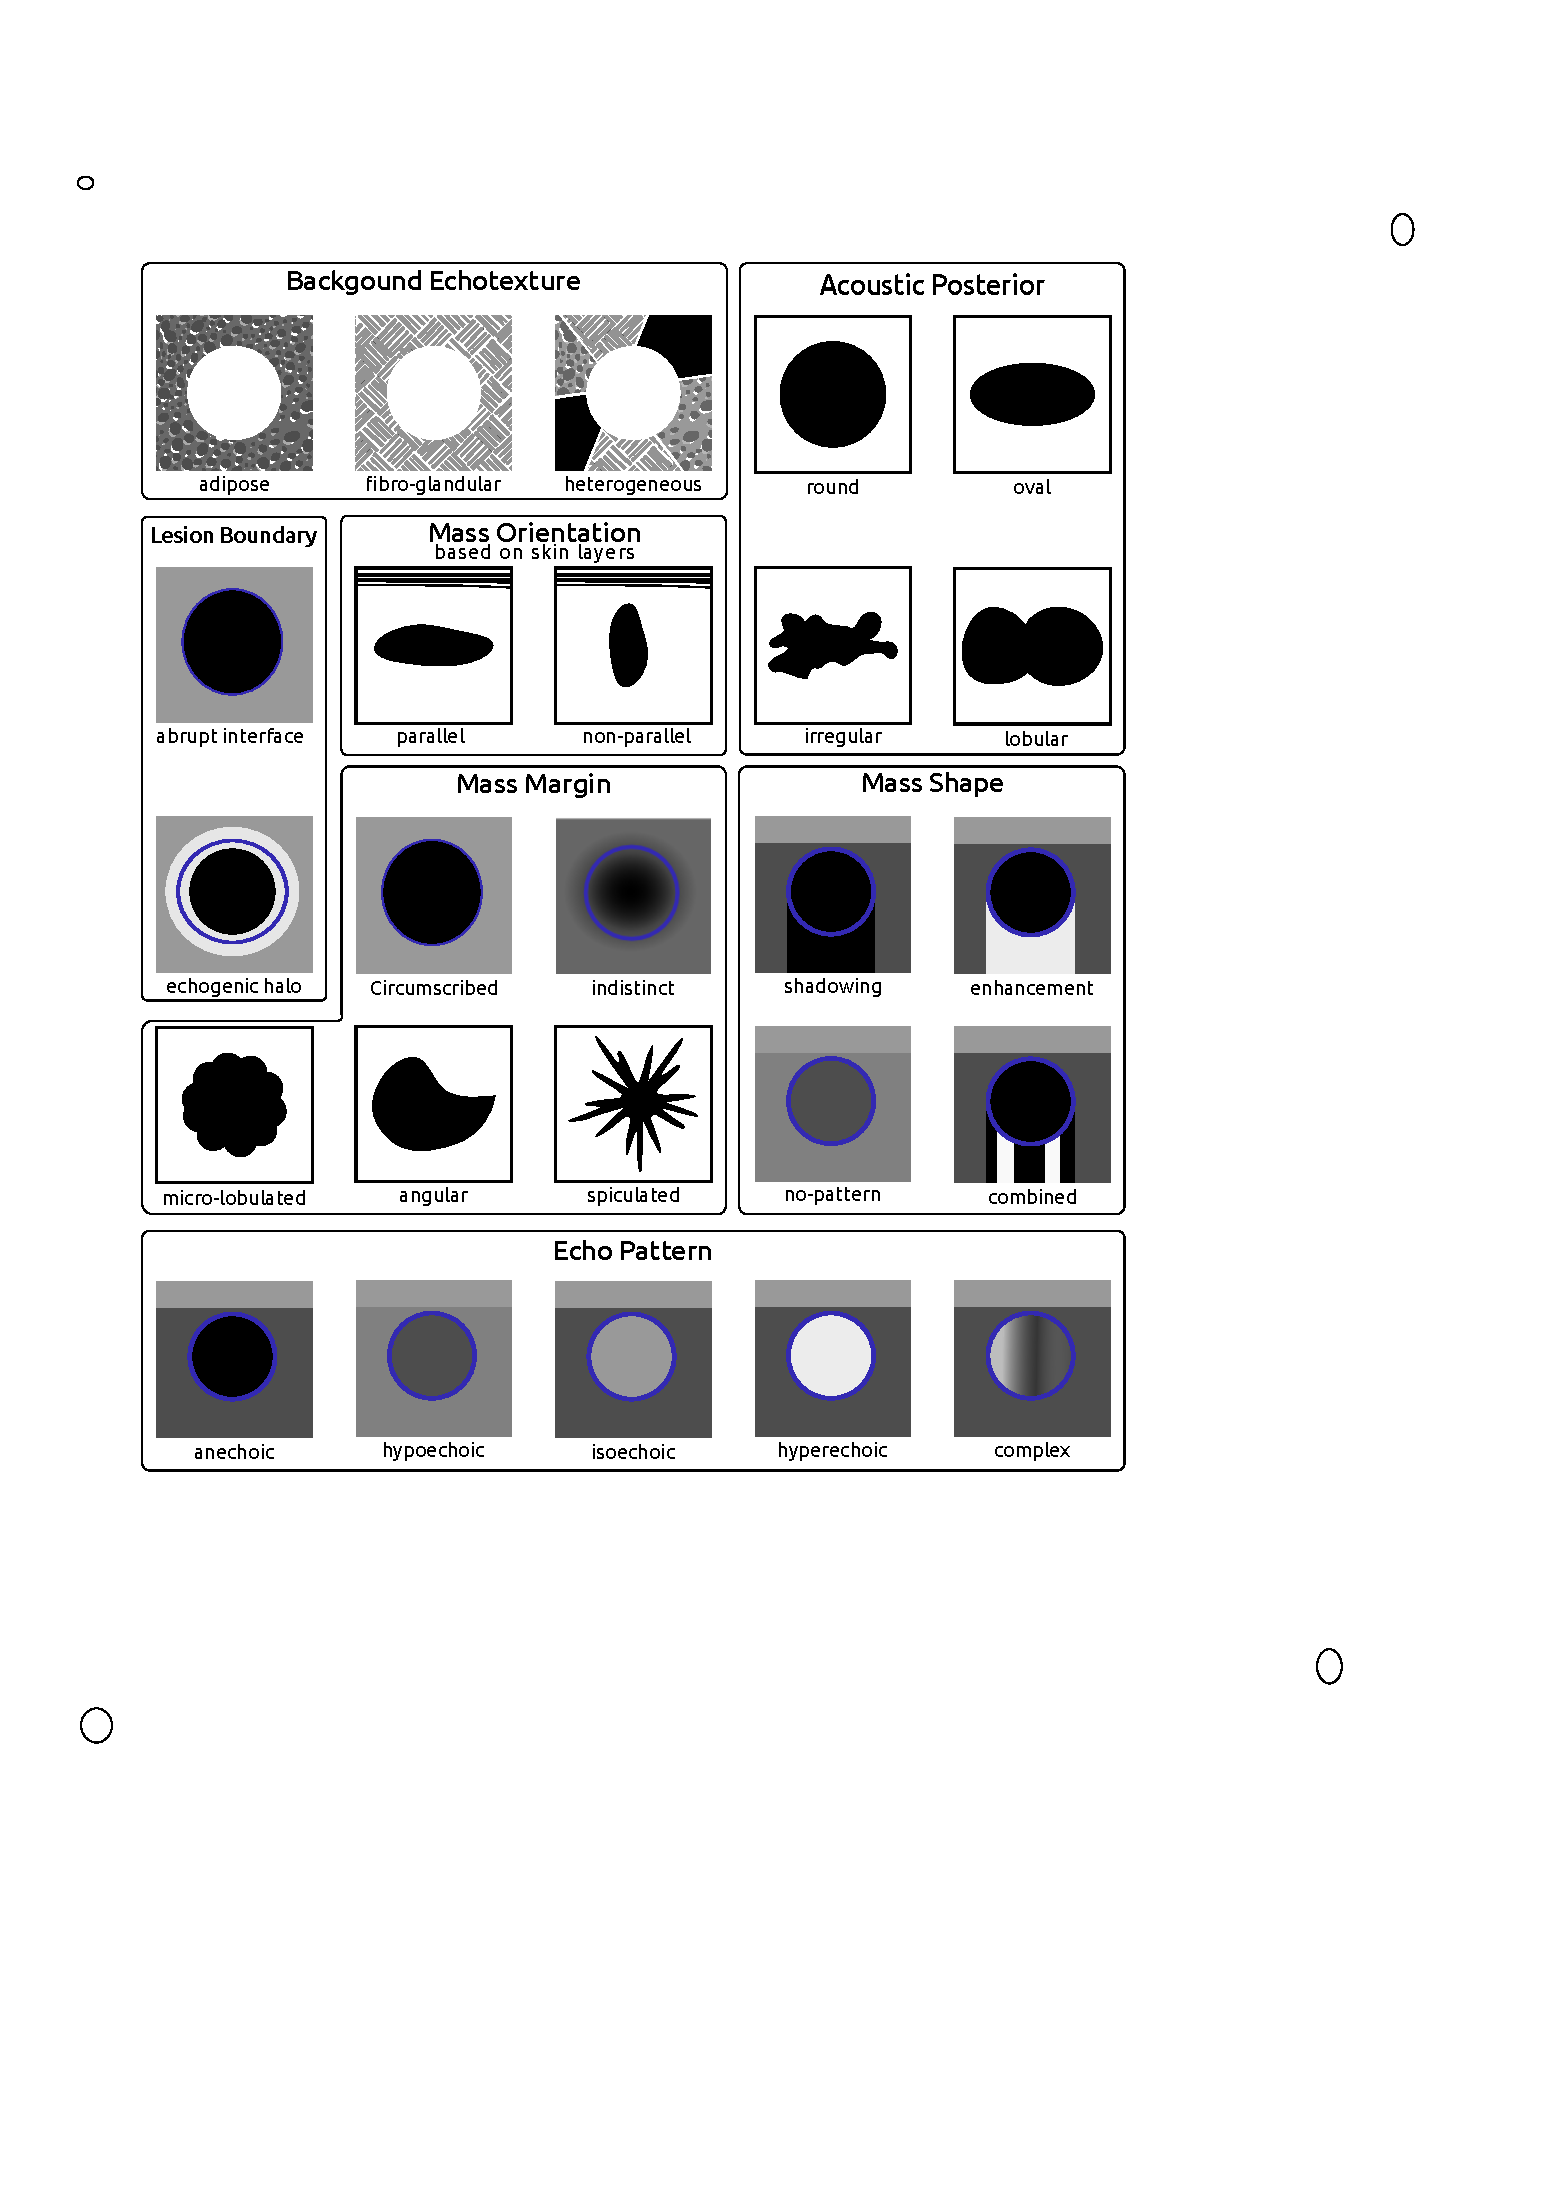
\includegraphics[trim = 65 345 200 124, clip,width=\textwidth]{birads}
        \caption[]%
        {Breast lesion characteristics in \ac{us} screening influencing clinical management~\cite{raza2010us}}
        \label{fig:lesions:lesions}
    \end{subfigure}
    \caption {{\small Visual reference of breast structures and visual cues used for standard \ac{bus} image assessment and diagnosis.}}
    \label{fig:lesions}
\end{figure}

When radiologists read an image to produce a diagnosis by analysing the markers, there is no need for an explicit delineation of the tissues or lesions present in the image since this is intrinsic to the reading process.
However, developing accurate segmentation methodologies breast lesions and structures is crucial for developing \ac{cad} systems.

%Regardless of the clinical utility of the \ac{us} images, such image modality suffers from different inconveniences due to strong noise natural of \ac{us} imaging  and the presence of strong \ac{us} artifacts, both degrading the overall image quality~\cite{Ensminger:2008p6920} which compromise the performance of the radiologists.
%Radiologists infer health state of the patients based on visual inspection of images which by means of some screening technique (e.g.~\ac{us}) depict physical properties of the screened body.
%The radiologic diagnosis error rates are similar to those found in any other tasks requiring human visual inspection, and such errors, are subject to the quality of the images and the ability of the reader to interpret the physical properties depicted on them\cite{manning2005perception}.
%
%Therefore the interest from the medical imaging community, also for the specific case of breast lesion assessment using \ac{us} data, in developing \ac{cad} systems that provide better instrumentation to improve image interpretation, and consequently achieve better diagnosis.

This article proposes a highly modular and flexible framework for segmenting lesions and tissues present in \ac{bus} images.
The proposal takes advantage of an energy-based strategy to perform segmentations based on discrete optimization using super-pixels and a set of novel features analogous to the elements present in \cref{fig:lesions}.

%%% Local Variables:
%%% mode: latex
%%% TeX-master: "../../master.tex"
%%% End: \section{introduction}
